\section{Local Air Temperature and SIC Correlations}
Firstly we are interested in looking at local effects on the behaviour of sea ice. We do this by taking the correlation between SIC values from the NSIDC dataset and 2m temperature reanalysis values for each gridpoint we have in our dataset. Because the datasets are on different grids, the temperature data has been interpolated to the same grid as the sea ice dataset here.
\begin{figure}[H]
    \centering
    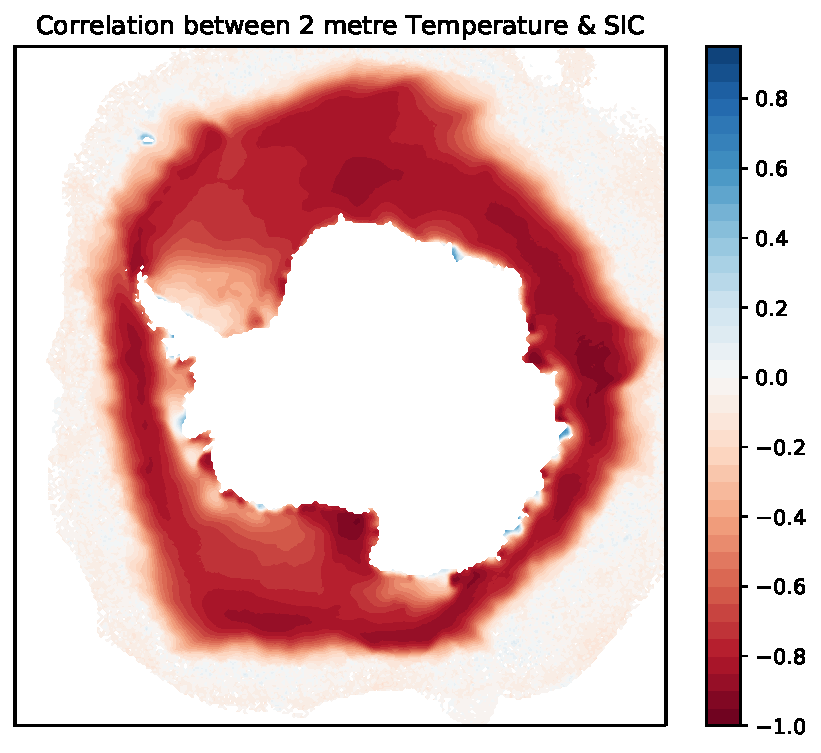
\includegraphics{Images/tempcorrwithsic.pdf}
    \caption{Correlation between temperature at 2m with sea ice concentration.}
    \label{fig:results:2mtemp_corr_with_sic}
\end{figure}

Above we have the correlation between 2 metre air temperature and sea ice concentration over Antarctica. The result that the temperature is negatively correlated with the concentration of sea ice in Antarctica is hardly surprising. Higher temperatures will be associated in the melting of ice. This both intuitively makes sense and is supported by the first law of thermodynamics (Conservation of energy). The main feature of interest in this plot is the regions which are close to the pole and there are lower correlations between 2m-temperature and SIC. It is possible that this is due to low variability in SIC in these regions over the entirety of each year.
